
%\cleardoublepage
\section{Kinematische Fahrzeugmodelle}\label{sec:VehicleKinematics}

In diesem Abschnitt werden kinematische Bewegungsmodelle zur Simulation von Fahrzeugen
eingeführt. Da sich diese Arbeit nicht auf ein spezifisches Fahrzeug fokussiert,
sondern allgemeine Erkenntnisse über die effiziente Erlernbarkeit von Fahrverhaltensweisen
mit einer Vielzahl verschiedenster Fahrzeuge liefern soll, werden zwei sehr
grundlegende Kinematiken anhand des Fahrradmodells und der Differential Drive Kinematik
vorgestellt. Die folgenden Informationen stammen aus dem Buch
\glqq{}Wheeled mobile robotics: from fundamentals towards autonomous systems\grqq{} \cite{klancar_2017_motion} und beziehen sich auf dessen Abschnitte 2.2.1 und 2.2.2.

\subsection{Kinematisches Fahrradmodell}\label{sec:Bicycle}
Das Fahrradmodell beschreibt die Bewegung eines Zweiradfahrzeugs mit Vorder-
und Hinterachse, wobei die Lenkung durch eine Drehung des Vorderrads um die z-Achse
des Koordinatensystems erreicht wird. Es können auch herkömmliche Automobile mit
Vorder- und Hinterachse durch das Fahrradmodell abgebildet werden, wenn vereinfachend davon
ausgegangen wird, dass sich auf beiden Achsen jeweils nur ein Rad in der Mitte befindet.
Für eine idealisierte Simulation wird außerdem angenommen, dass es keinen
Reibungswiderstand gibt und dass sich das Fahrzeug in einer flachen 2D Ebene bewegt.\\

\begin{figure}[h]
  \centering
  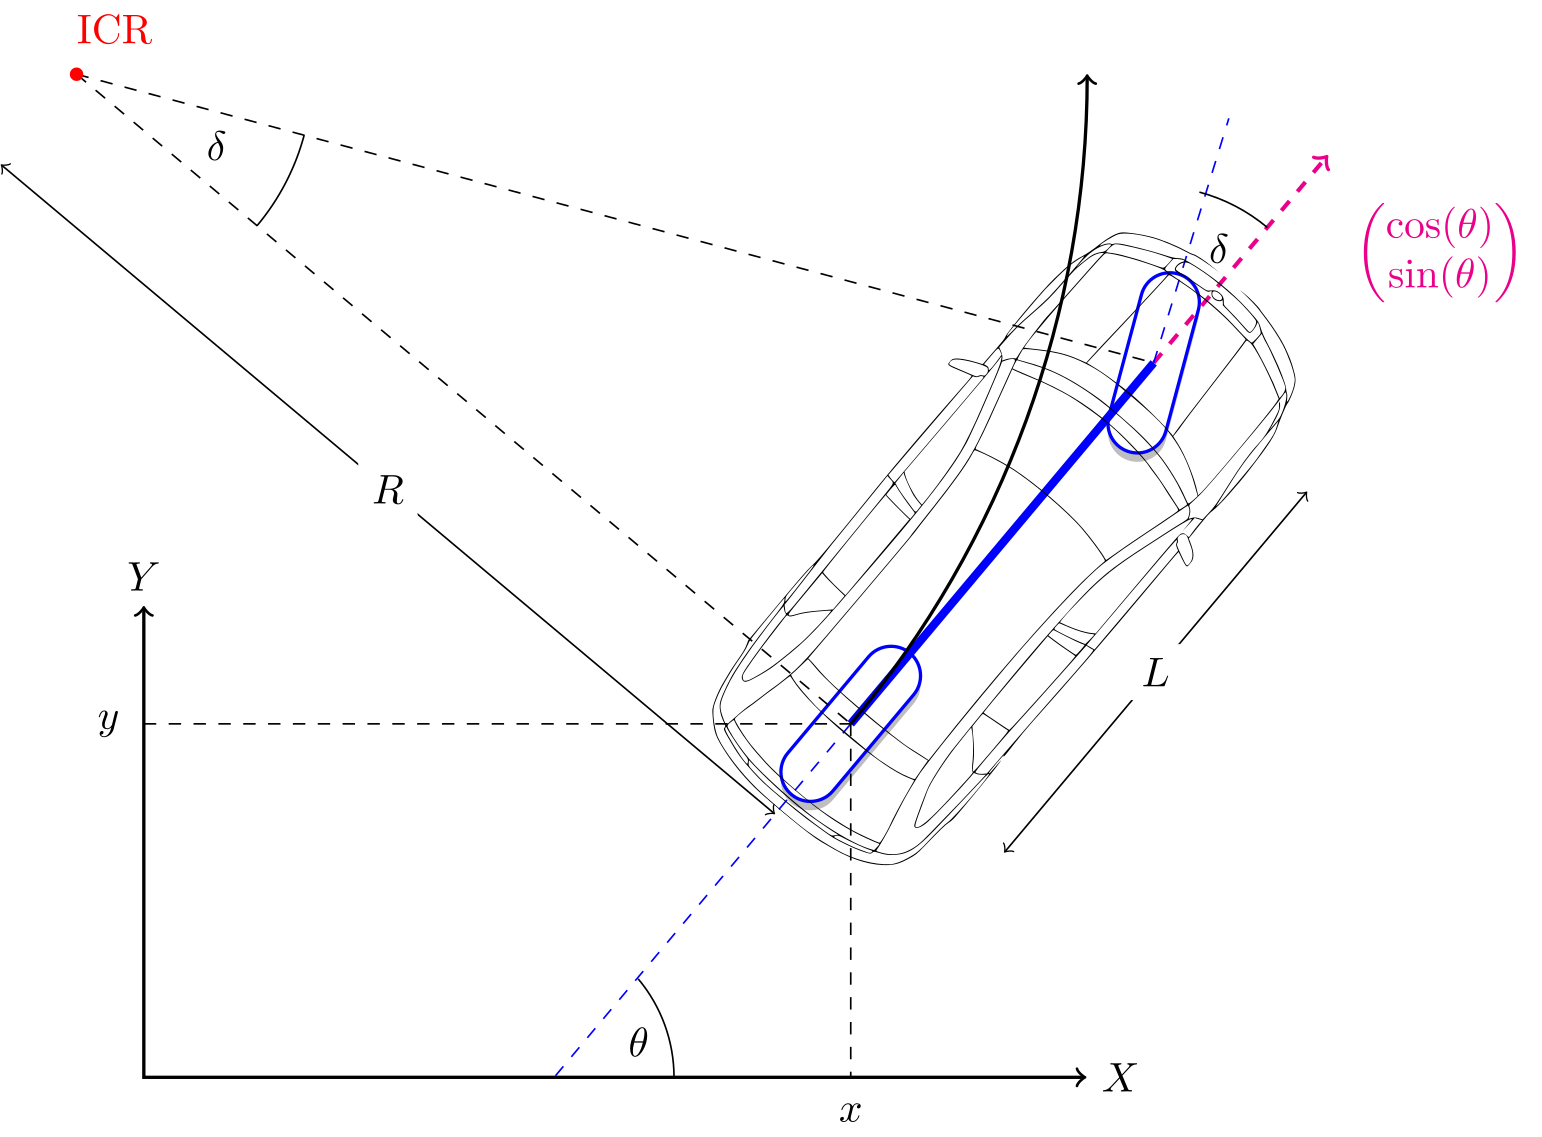
\includegraphics[width = 0.65\textwidth]{imgs/bicycle_model}
  \caption{Skizze des kinematischen Fahrradmodells \cite{fermi2023bicycleimg}}
  \label{img:BicycleDrive}
\end{figure}

Wie in Abbildung \ref{img:BicycleDrive} zu sehen ist, befindet sich das Fahrzeug mit dem
Hinterrad an der Position $(x, y)^T$ und hat das Vorderrad um den Lenkwinkel $\delta$
eingeschlagen. $L$ beschreibt die Distanz zwischen Vorder- und Hinterachse, $\theta$
die Ausrichtung, $v$ die Geschwindigkeit und $a$ die Beschleunigung des Fahrzeugs.
$\Delta \theta$ repräsentiert hingegen die Winkelgeschwindigkeit, mit der sich das Fahrzeug
auf seiner Kreisbahn um den Momentanpol bewegt. Die Berechnung des neuen Fahrzeugzustands
nach $\Delta t$ kann mit folgenden Gleichungen formalisiert werden:

\begin{equation}
\begin{aligned}
\frac{d}{dt} \begin{pmatrix} x \\ y \\ \theta \\ v \end{pmatrix}
= \begin{pmatrix} v \cdot cos(\theta) \\ v \cdot sin(\theta)
    \\ v \cdot \frac{tan(\delta)}{L} \\ a \end{pmatrix}
\end{aligned}
\end{equation}

Anhand der neuen Geschwindigkeit und Ausrichtung des Fahrzeugs wird dessen gerichtete
Bewegungsdynamik bestimmt. Der Fahrer steuert durch die Vorgabe der Beschleunigung $a$
und des Lenkwinkels $\delta$. Als Repräsentation des aktuellen Fahrzeugzustands dienen
die Geschwindigkeit $v$ und der Lenkwinkel $\delta$.

\subsection{Differential Drive}\label{sec:DiffDrive}
Bei der Differential Drive Kinematik wird von einem Fahrzeug
ausgegangen, dessen linke und rechte Räder unabgängig voneinander drehen können.
Indem die Räder auf beiden Seiten entgegengesetzt drehen, kann sich das Fahrzeug
auf der Stelle drehen. Eine Lenkung wird erzielt, indem sich die Räder auf der
kurvenabgewandten Seite schneller drehen. Auch hier wird idealisierend angenommen,
dass sich das Fahrzeug in einer flachen 2D Ebene bewegt und es keinen
Reibungswiderstand gibt.\\

\begin{figure}[h]
  \centering
  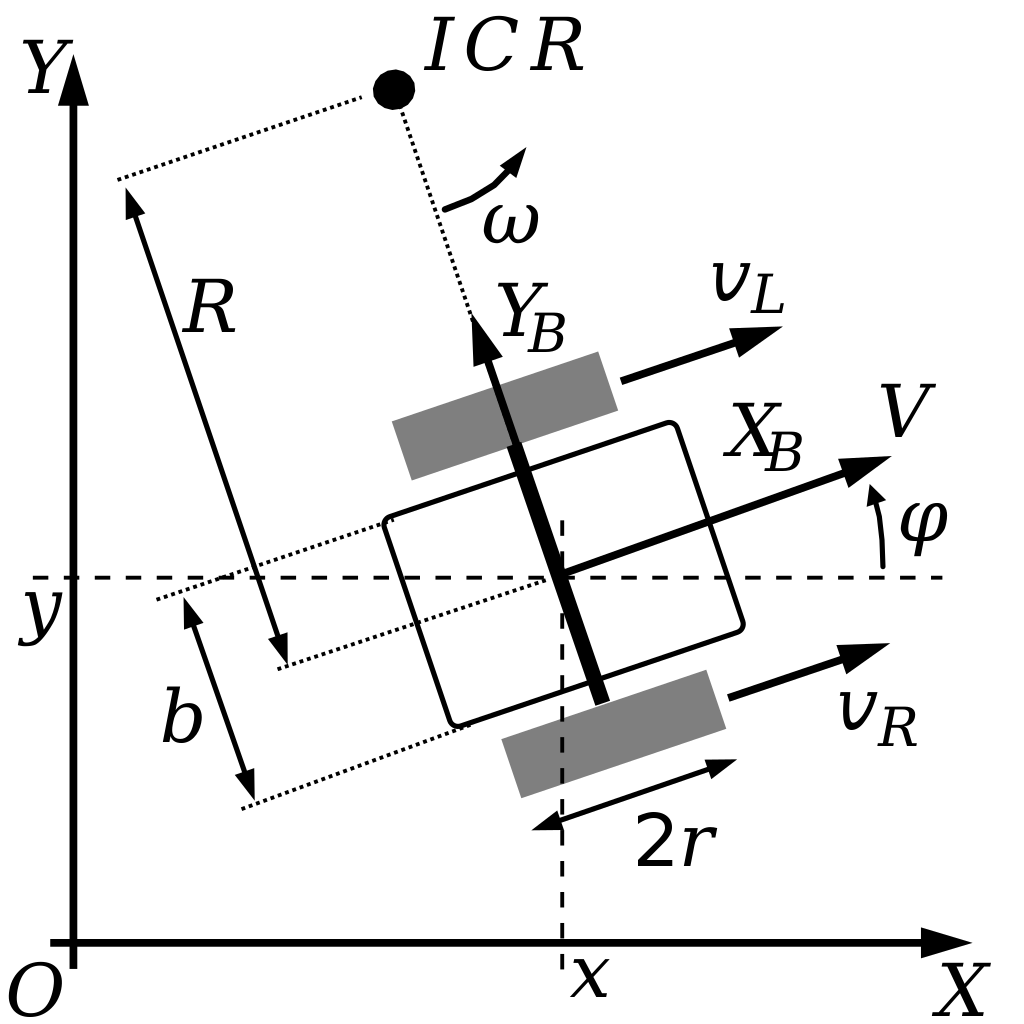
\includegraphics[width = 0.65\textwidth]{imgs/diff_drive}
  \caption{Skizze der Differential Drive Kinematik, \cite{mrdrno2023diffdriveimg}}
  \label{img:DiffDrive}
\end{figure}

Wie in Abbildung \ref{img:DiffDrive} dargestellt, befindet sich die Fahrzeugbasis
$(x, y)^T$ in der Mitte der auf einer Achse aufgehängten, unabhängig voneinander
drehbaren Räder mit Radius $r$. $\varphi$ beschreibt die Ausrichtung des Fahrzeugs
im Koordinatensystem und $\omega$ repräsentiert die Winkelgeschwindigkeit, mit der
sich das Fahrzeug auf seiner Kreisbahn um den Momentanpol mit Geschwindigkeit $v$
dreht. Die Räder rotieren mit den Rotationsgeschwindigkeiten $\omega_R$ und $\omega_L$
um ihre Achse der Breite $b$ und legen pro Umdrehung eine Strecke in Höhe ihres
Umfangs von $2r\pi$ zurück. Mit $x_B$ und $y_B$ wird die zum Fahrzeug relative
Bewegung nach vorne bzw. zur Seite beschrieben. Folgende Gleichungen modellieren
die Differential Drive Kinematik:

\begin{equation}
\begin{aligned}
\frac{d}{dt} \begin{pmatrix} x_B \\ y_B \\ \varphi \end{pmatrix}
= \begin{pmatrix} v \cdot x_B \\ v \cdot y_B \\ \omega \end{pmatrix}
= \begin{pmatrix} \frac{r}{2} \cdot (\omega_R + \omega_L) \\ 0
     \\ \frac{r}{b} \cdot (\omega_R - \omega_L) \end{pmatrix}
\end{aligned}
\end{equation}

Für eine erleichterte Steuerung gibt der Fahrer die Geschwindigkeit $V$ und
Winkelgeschwindigkeit $\omega$ vor, die anschließend in die passenden
Rotationsgeschwindigkeiten $\omega_R$ und $\omega_L$ der Räder übersetzt werden,
um eine entsprechende Bewegung zu erzielen. Als Repräsentation des aktuellen
Fahrzeugzustands dienen die zur Fahrzeugausrichtung relative Vorwärtsbewegung $x_B$
und die Winkelgeschwindigkeit $\omega$.

\begin{equation}
\begin{aligned}
\omega_R = \frac{2V + \omega b}{2r}, \omega_L = \frac{2V - \omega b}{2r}
\end{aligned}
\end{equation}

\begin{equation}
\begin{aligned}
\frac{d}{dt} \begin{pmatrix} x \\ y \\ \varphi \end{pmatrix}
= \begin{pmatrix} V \cdot cos(\varphi) \\ V \cdot sin(\varphi) \\ \omega \end{pmatrix}
\end{aligned}
\end{equation}

Bei der Modellierung der resultierenden Bewegung ergibt sich im Vergleich zum
Fahrradmodell eine sehr ähnliche Kinematik, wobei $V = v$ und $\varphi = \theta$
entspricht.
